\section{Meccanismi di controllo e rendicontazione}
Sono stati predisposti metodi per il controllo delle attività e per la rendicontazione delle ore impiegate nello svolgimento di tali attività. Tali meccanismi servono principalmente al \emph{Responsabile} di progetto per avere una chiara visione dell'andamento del progetto.
\subsection{Meccanismi di controllo}
\subsubsection{Controllare l'andamento delle attività}

Tramite la piattaforma di ticketing adottata, descritto nelle \NormeDiProgetto, è possibile visualizzare in modo semplice l'\textbf{andamento delle attività}.
Nella schermata Task, visibile nella figura \ref{teamworkpmtask} vengono indicati tutti task, correlati di attività con
\begin{itemize}
\item La percentuale di \textbf{completamento} delle attività aperte;
\item Le attività in \textbf{ritardo}, indicate in rosso;
\item Le attività \textbf{concluse}, modificando i filtri di visualizzazione.
\end{itemize}
 
\begin{figure}[H]
\centering 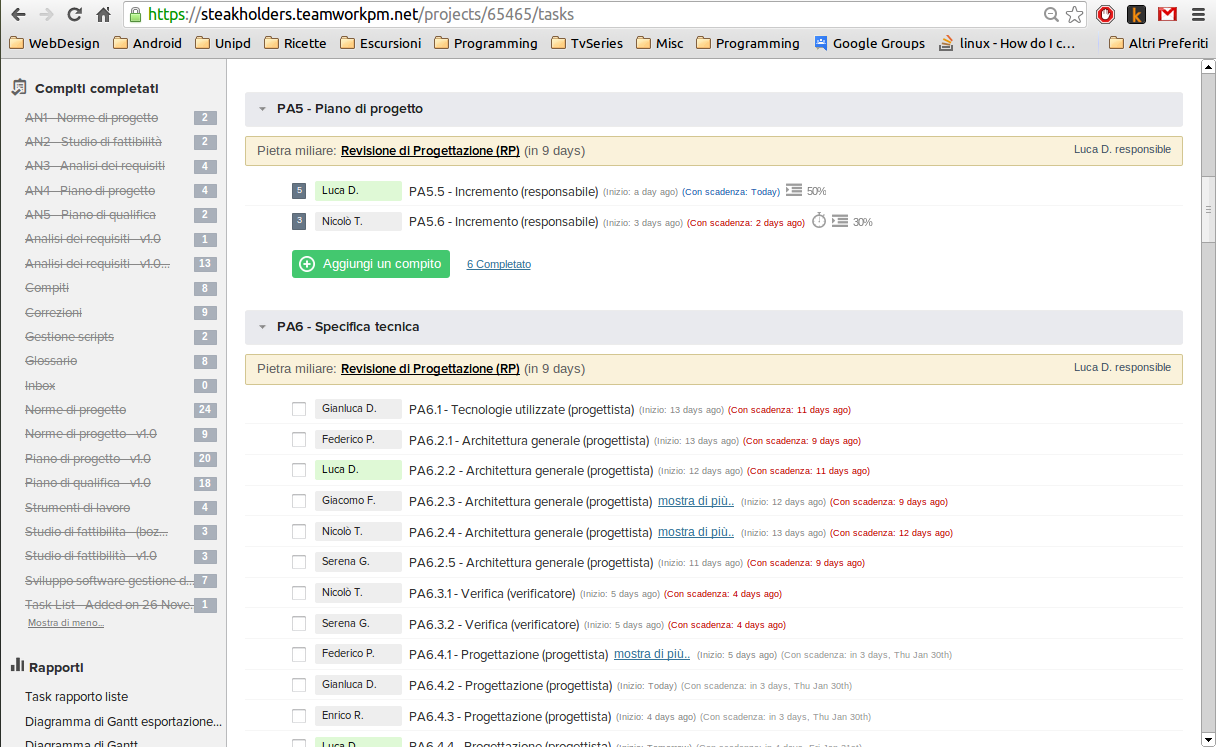
\includegraphics[scale=0.3]{gantt/task-list.png}
\caption{Schermata task di \glossario{TeamworkPM} \label{teamworkpmtask}}
\end{figure}


\subsubsection{Permettere un aggiornamento facilitato della pianificazione}
\label{script}
È impensabile che ad ogni raffinamento del Piano di lavoro il \emph{Responsabile} e l' \emph{Amministratore} riscrivano a mano le sezioni interessate del \PianoDiProgetto.
Per questa ragione è fondamentale che, una volta aggiornata la piattaforma di ticketing\footnote{Vedi \NormeDiProgetto}, i documenti vengano \textbf{aggiornati in modo automatizzato}.

Tale obiettivo è stato implementato con uno script che preleva i dati necessarie dal \glossario{TeamworkPM} e genera le tabelle, i diagrammi di \glossario{Gantt} e i grafici necessari per il \PianoDiProgetto.

\subsection{Meccanismi di rendicontazione}

Incrementando gli script descritti nella sezione \ref{script} è possibile rendicontare le ore effettive consumate per completare le attività stabilite.
Tale ore sono calcolate confrontando le ore stimate nel \PianoDiProgetto{} sezione \ref{pianificazione} con quelle effettivamente impiegate, indicate su \glossario{TeamworkPM}.
Per una visione immediata sono state incluse nel capitolo \ref{capitolosuddivisionelavoro}.


